\documentclass[a4paper,fleqn,usenatbib]{mnras}

% MNRAS is set in Times font. If you don't have this installed (most LaTeX
% installations will be fine) or prefer the old Computer Modern fonts, comment
% out the following line
% \usepackage{newtxtext,newtxmath}
\usepackage{times}
% Depending on your LaTeX fonts installation, you might get better results with one of these:
% \usepackage{mathptmx}
% \usepackage{txfonts}

% Use vector fonts, so it zooms properly in on-screen viewing software
% Don't change these lines unless you know what you are doing
\usepackage[T1]{fontenc}
\usepackage{ae,aecompl}

%%%%% AUTHORS - PLACE YOUR OWN PACKAGES HERE %%%%%
%\usepackage{epsf}
\usepackage{color}
\usepackage{graphicx}
\usepackage{amsmath}	% Advanced maths commands
\usepackage{amssymb}	% Extra maths symbols
\usepackage{natbib}
%\usepackage[colorlinks,urlcolor=blue,citecolor=blue,linkcolor=blue]{hyperref}
\usepackage{multirow}
\usepackage{etoolbox}

%%%%% AUTHORS - PLACE YOUR OWN COMMANDS HERE %%%%%
%%% Fields %%%
\newcommand{\hdf}{HDF-N}
\newcommand{\hdfn}{HDF-N}
\newcommand{\hdfs}{HDF-S}
\newcommand{\cdfs}{CDF-S}

%%% Telescopes %%%
\newcommand{\hst}{\textit{HST}}
\newcommand{\iras}{\textit{IRAS}}
\newcommand{\iso}{\textit{ISO}}
\newcommand{\spitzer}{\textit{Spitzer}}
\newcommand{\sirtf}{\textit{Spitzer}}
\newcommand{\chandra}{\textit{Chandra}}

%%% Filters %%%
\newcommand{\wfu}{\hbox{$\mathrm{U}_{300}$}}
\newcommand{\wfb}{\hbox{$\mathrm{B}_{450}$}}
\newcommand{\wfv}{\hbox{$\mathrm{V}_{606}$}}
\newcommand{\wfi}{\hbox{$\mathrm{I}_{814}$}}
\newcommand{\acsb}{\hbox{$\mathrm{B}_{435}$}}
\newcommand{\acsv}{\hbox{$\mathrm{V}_{606}$}}
\newcommand{\acsi}{\hbox{$i_{775}$}}
\newcommand{\acsz}{\hbox{$z_{850}$}}
\newcommand{\nicj}{\hbox{$\mathrm{J}_{110}$}}
\newcommand{\nich}{\hbox{$\mathrm{H}_{160}$}}
\newcommand{\wfcy}{\hbox{$\mathrm{Y}_{105}$}}
\newcommand{\wfcj}{\hbox{$\mathrm{J}_{125}$}}
%\newcommand{\wfcj}{\hbox{$J_{110}$}}
\newcommand{\wfch}{\hbox{$\mathrm{H}_{160}$}}
\newcommand{\sdssu}{\hbox{$u$}}
\newcommand{\sdssg}{\hbox{$g$}}
\newcommand{\sdssr}{\hbox{$r$}}
\newcommand{\sdssi}{\hbox{$i$}}
\newcommand{\sdssz}{\hbox{$z$}}
\newcommand{\mone}{\hbox{$[3.6]$}}
\newcommand{\mtwo}{\hbox{$[4.5]$}}
\newcommand{\mthree}{\hbox{$[5.8]$}}
\newcommand{\mfour}{\hbox{$[8.0]$}}
%\newcommand{\mone}{\hbox{$[3.6\mu\mathrm{m}]$}}
%\newcommand{\mtwo}{\hbox{$[4.5\mu\mathrm{m}]$}}
%\newcommand{\mthree}{\hbox{$[5.8\mu\mathrm{m}]$}}
%\newcommand{\mfour}{\hbox{$[8.0\mu\mathrm{m}]$}}

%%% Astronomy Abreviations %%%
\newcommand{\mstar}{\hbox{$\mathrm{M}^\ast$}}
\newcommand{\lstar}{\hbox{$L^\ast$}}
\newcommand{\Msol}{\hbox{$\mathrm{M}_\odot$}}
\newcommand{\msol}{\hbox{$\mathrm{M}_\odot$}}
\newcommand{\Zsol}{\hbox{$Z_\odot$}}
\newcommand{\zsol}{\hbox{$Z_\odot$}}
\newcommand{\Lsol}{\hbox{$L_\odot$}}
\newcommand{\lsol}{\hbox{$L_\odot$}}
\newcommand{\lir}{\hbox{$L_{\mathrm{IR}}$}}
\newcommand{\zph}{\hbox{$z_\mathrm{ph}$}}
\newcommand{\zphot}{\hbox{$z_\mathrm{ph}$}}
\newcommand{\lbol}{\hbox{$L_\mathrm{bol}$}}
\newcommand{\snr}{\hbox{$\mathrm{S/N}$}}
\newcommand{\reff}{\hbox{$r_\mathrm{eff}$}}
\newcommand{\ks}{\hbox{$K_s$}}
\newcommand{\AAA}{\hbox{\AA}}

%%% Spectrum Lines %%%
\newcommand{\lya}{ Ly$\alpha \;$}
\newcommand{\lyb}{Lyman~$\beta$}
\newcommand{\hb}{\hbox{H$\beta$}}
\newcommand{\ha}{\hbox{H$\alpha$}}
\newcommand{\paa}{\hbox{Pa$\alpha$}}

%%% Units %%%
\newcommand{\kms}{\hbox{km~s$^{-1}$}}
\newcommand{\cms}{\hbox{cm~s$^{-1}$}}
\newcommand{\mpc}{\hbox{Mpc$^{-1}$}}
\newcommand{\mpcsq}{\hbox{Mpc$^{-2}$}}
\newcommand{\mpccu}{\hbox{Mpc$^{-3}$}}
\newcommand{\cnts}{\hbox{cnt~s$^{-1}$}} 
\newcommand{\cmsq}{\hbox{cm$^{-2}$}}
\newcommand{\cmcu}{\hbox{cm$^{-3}$}}
\newcommand{\ergscm}{\hbox{erg~s$^{-1}$~cm$^{-2}$}}
\newcommand{\uJy}{\hbox{$\mu$Jy}}
\newcommand{\ujy}{\hbox{$\mu$Jy}}
\newcommand{\degree}{\hbox{$^\circ$}}
\newcommand{\degsq}{\hbox{degree$^2$}}
\newcommand{\arcminsq}{\hbox{arcmin$^2$}}
\newcommand{\um}{\hbox{$\mu$m}}

%%% Math %%%
\newcommand{\lsim}{\lesssim}
\newcommand{\gsim}{\gtrsim}
\newcommand{\mathS}{\hbox{$\mathcal{S}$}}
\newcommand{\mathR}{\hbox{$\mathcal{R}$}}
\newcommand{\mathM}{\hbox{$\mathcal{M}$}}
\newcommand{\mcal}{\hbox{$\mathcal{M}$}}
\newcommand{\rcal}{\hbox{$\mathcal{R}$}}
\newcommand{\scal}{\hbox{$\mathcal{S}$}}
\newcommand{\infinity}{\hbox{$\infty$}}
\newcommand{\err}[2]{$^{+#2}_{-#1}$}

%%% General %%%
\newcommand{\etal}{et al.}
\newcommand{\eg}{e.g.}
\newcommand{\ie}{i.e.}
\newcommand{\cf}{cf.}
% \newcommand{\ion}[2]{\hbox{#1$\;${\small\rm{#2}}}}
\newcommand{\mybullet}{\noindent$\bullet$}
\newcommand{\uit}{\textit{UIT}}
\newcommand{\nd}{...}
%\newcommand{\cmodel}{\hbox{\tt cmodel}}
%\newcommand{\bs}{\hbox{$\!\!\!\!$}}
\newcommand{\todo}[1]{{\tt #1}}
\newcommand{\citeeg}[1]{(\eg, \citealt{#1})}
\newcommand{\ignore}[1]{}

%%% Extra %%% 
% \newcommand{\farcm}{\mbox{\ensuremath{.\mkern-4mu^\prime}}}%fractional arcminute symbol 0.'0
% \newcommand{\farcs}{\mbox{\ensuremath{.\!\!^{\prime\prime}}}}%fractional arcsecond symbol: 0.''0
% \newcommand{\fdg}{\mbox{\ensuremath{.\!\!^\circ}}}%fractional degree symbol:     0.°0
\newcommand{\arcdeg}{\ensuremath{^{\circ}}}%                    % degree symbol:  °
% \newcommand{\sun}{\ensuremath{\odot}}%                          % sun symbol
% \newcommand{\apj}{ApJ}%                                         % Journal abbreviations
% \newcommand{\apjs}{ApJS}
% \newcommand{\apjl}{ApJL}
% \newcommand{\aap}{A{\&}A}
% \newcommand{\aaps}{A{\&}AS}
% \newcommand{\mnras}{MNRAS}
% \newcommand{\aj}{AJ}
% \newcommand{\araa}{ARAA}
% \newcommand{\pasp}{PASP}
\newcommand{\Teff}{\ensuremath{T_{\mathrm{eff}}}}%              % T_eff
\newcommand{\logg}{\ensuremath{\log g}}%                        % log g
\newcommand{\bv}{\ensuremath{B\!-\!V}}%                         % B-V
\newcommand{\ub}{\ensuremath{U\!-\!B}}%                         % U-B
\newcommand{\vr}{\ensuremath{V\!-\!R}}%                         % V-R
\newcommand{\ur}{\ensuremath{U\!-\!R}}%                         % U-R

\newcommand{\editorial}[1]{\textcolor{red}{#1}}
\DeclareRobustCommand{\ion}[2]{%
\relax\ifmmode
\ifx\testbx\f@series
{\mathbf{#1\,\mathsc{#2}}}\else
{\mathrm{#1\,\mathsc{#2}}}\fi
\else\textup{#1\,{\mdseries\textsc{#2}}}%
\fi}

%%%%%%%%%%%%%%%%%%% TITLE PAGE %%%%%%%%%%%%%%%%%%%
\title[Short Title]{Cluster Dynamics with HETDEX - I: Simulated Performance, Mass Distribution and Limits}

% The list of authors, and the short list which is used in the headers.
% If you need two or more lines of authors, add an extra line using \newauthor
\author[S. Boada et al.]{
Steven Boada,$^{1}$\thanks{E-mail: boada@physics.tamu.edu}
C.~Papovich,$^{1}$
R.~Wechsler,$^{2,3}$
T. S.~Li,$^{1}$\newauthor\phantom{x}
K.~Gebhardt,$^{4}$
E.~Rozo,$^{2}$
E. S.~Rykoff,$^{2}$
\\
% List of institutions
$^{1}$George P.\ and Cynthia Woods Mitchell Institute for
Fundamental Physics and Astronomy, Texas A\&M University, College Station, TX, 77843-4242\\
$^{2}$Kavli Institute for Particle Astrophysics and Cosmology, Department of Physics, Stanford University, Stanford, CA 94305, USA\\
$^{3}$Department of Particle Physics and Astrophysics, SLAC National Accelerator Laboratory, Menlo Park, CA 94025, USA\\
$^{4}$The University of Texas}

% These dates will be filled out by the publisher
\date{Accepted XXX. Received YYY; in original form ZZZ}

% Enter the current year, for the copyright statements etc.
\pubyear{2016}

% Don't change these lines
\begin{document}
\label{firstpage}
\pagerange{\pageref{firstpage}--\pageref{lastpage}}
\maketitle

\begin{abstract}
\noindent
The study of clusters of galaxies has been argued to be a very effective way to measure cosmological parameters, including measuring dark energy and testing models of gravity. The Hobby Eberly Telescope Dark Energy Experiment (HETDEX) will observe many hundreds of square degrees, covering a large sample of galaxy clusters out to $z = 0.5$ based on their optical spectra ($3500-5500\AAA$). The spectra will provide important measures of the clusters dynamics and may enable constraints on cosmological parameters, but only if the measurements provide accurate estimates of the total cluster masses. We have carried out a study to investigate the ability of HETDEX to recover accurate galaxy cluster masses over a wide range of masses and redshifts. We used a detailed mock galaxy catalog and present mock observations of two different scenarios: (1) We targeted individual galaxy clusters to investigate the recovery of parameters with such observations. (2) We created and evaluated a HETDEX-like selection "function'' of galaxies over a similarly sized portion of the sky and use well adopted techniques to recover the dynamical properties, such as velocity dispersion and mass. Using both observing strategies, we produce cluster mass probability density functions $P(X|M,z)$, which can be used to determine the probability that a galaxy cluster of given mass (M), located at redshift ($z$) determined using observable parameter (X). 
% We then applied these probability functions to ten galaxy clusters selected from the Sloan Digital Sky Survey DR8 and the Chandra-XMM X-ray Cluster Survey at $z=0.2-0.3$, and observed by the HETDEX spectrograph prototype instrument (VIRUS-p). We measured spectroscopic redshifts and line-of-sight velocities of the galaxies in and around each cluster, derived a line-of-sight velocity dispersion, and inferred a dynamical mass for each cluster which ranges from $(0.4-24) \times 10^{14} \Msol (M_{200c})$. Using the mass probability density functions described above, we updated these masses and compared them to existing literature estimates, or to the masses estimated from other observables such as X-ray temperature or richness.
\end{abstract}

\section{INTRODUCTION}
Our ability to perform precision cosmology with clusters of galaxies has reached a critical turning point. The widely accepted $\Lambda$CDM model of cosmology makes explicit predictions about the number and masses of galaxy clusters throughout the universe. However, connecting these predictions to a set of, sufficiently large in size, observed clusters remains a principal problem. Specifically, the largest threat to modern, precision, cluster cosmology is not the identification of large numbers of clusters (the total number of clusters known is only going up) but the accurate recovery of galaxy cluster mass \citeeg{Sehgal2011,Plank2014, Bocquet2015}.

As mass is not a direct observable, a lot of work is underway to characterize galaxy cluster masses with an observable feature of galaxy clusters. The goal is to constrain, as best possible, $P(X|M,z)$ the probability ($P$) that a galaxy cluster of given mass ($M$), located at redshift ($z$) determined using observable parameter ($X$). The observable parameter most commonly observed X-ray temperatures and luminosities \citeeg{Mantz2010, Rykoff2014, Mantz2015}, cosmic microwave background observations \citeeg{Vanderlinde2010, Sehgal2011} using the Sunyaev-Zel'dovich effect (SZE; \citealt{Sunyaev1972}) or optical studies \citeeg{Rozo2010, Rozo2015} of richness \citeeg{Abell1958, Rykoff2012} or galaxy velocity dispersions \citeeg{Ruel2014, Sifon2015}.

Massive surveys, both on going and planned, are revolutionizing cluster cosmology using a large range of wavelengths. The South Pole Telescope (SPT; \citealt{Carlstrom2011}) and the Atacama Cosmology Telescope (ACT; \citealt{Swetz2011}) are discovering many clusters through the SZE. Optically, the on going The Dark Energy Survey (DES; \citealt{DES2005}) and planned Large Synoptic Survey Telescope (LSST; \citealt{LSST2012}) will identify many thousands of clusters to much lower masses than is possible with SZE measurements. However, regardless of the discovery method used, spectroscopic followup is needed to further constrain $P(X|M,z)$. But as the cluster dataset grows to many tens of thousands of clusters individual followup becomes increasingly impractical. Therefore, large spectroscopic surveys are needed to more fully constrain the observable--mass relation of clusters.

The Hobby Eberly Telescope Dark Energy eXperiment (HETDEX; \citealt{Hill2008}) is a trailblazing effort to observe high-redshift large scale structures using cutting edge wide-field integral field unit (IFU) spectrographs. Designed to probe the evolution of the dark energy equation of state etched onto high redshift ($z>2$) galaxies by the Baryon Acoustic Oscillations \citep{Eisenstein2005} in the first moments of the universe, the survey will observe two fields for a total of 420 \degsq\ from two fields (300 \degsq, Spring field and 120 \degsq, Fall field). Tuned to find \lya\ emitting (LAE) galaxies at $1.9<z<3.5$, HETDEX expects to find 800,000 LAEs, and more than one million [\ion{O}{ii}] emitting galaxies at $z<0.5$ masquerading as high-redshift galaxies \citep{Acquaviva2014}. 

While a large portion of the $\sim10^6$ interloping [\ion{O}{ii}] galaxies will be field (not associated with a bound structure) galaxies, the large area covered by HETDEX is expected to contain as many as 100 Virgo-sized ($M_{dyn}\sim 10^{15}$ \msol) clusters at $z<0.5$ (\editorial{citation?}). The near-complete spectroscopic coverage allows an unprecedentedly detailed look at a very large number of clusters ranging from group scales to the very massive. In addition to the recovery of accurate dynamical masses, detailed investigations of the of dynamical state of the clusters is possible. 

Connecting the dynamical properties derived from spectroscopy to the properties inferred from other studies insures the greatest impact on future work. HETDEX overlaps with the Sloan Digital Sky Survey (SDSS; \citealt{Blanton2001a}), SDSS stripe 82 \citep{Annis2014}, the Dark Energy Survey (DES; \citealt{DES2005}), and the upcoming DECam/IRAC Galaxy Environment Survey (DIRGES; PI: Papovich, C. Papovich \etal\ in preparation). \editorial{SHELA and others? Would be good to have a whole list of different things and different wavelengths.} While the potential dataset is very rich, two large issues remain.

It is unclear how a blind spectroscopic survey with an IFU will effect the recovery of galaxy cluster dynamical properties. Unlike many previous large cluster surveys \citeeg{Milvang-Jensen2008, Robotham2011, Sifon2015} which use multi-object spectrographs, the Visible Integral-Field Replicable Unit Spectrograph (VIRUS; \citealt{Hill2012}) used by HETDEX samples the sky unevenly which could excluded member galaxies which would otherwise be included. Secondly, it is not straightforward to use spectroscopic redshifts predominately from emission-line galaxies to interpret the kinematic and dynamical states of the clusters.

This work plans to address these concerns in the following ways. We use simulated observations which target individual galaxy clusters to investigate the recovery of parameters with such observations. Secondly, we create and evaluate a HETDEX like selection ``function'' of galaxies over a similarly large portion of the sky and use well adopted techniques to recover the dynamical properties, such as velocity dispersion and mass. Each observation strategy will further be constrained with ``ideal'' and ``realistic'' knowledge. Ideal knowledge assumes that we know which individual galaxy is assigned to which cluster. With realistic knowledge this is unknown and must be determined prior to the estimation of the cluster properties. Both of these strategies will better allow future work to predict the number and types of galaxy clusters which should be observed with VIRUS during both the HETDEX survey portion and through targeted follow up observations.

\editorial{Give outline of paper section.}

Throughout this paper, we adopt the following cosmological model ($\Omega_\Lambda = 0.77$,
$\Omega_M = 0.23$, $\sigma_8 = 0.83$ and $H_0= 72$ \kms \mpc), assume a Chabrier initial mass function (IMF; \citealt{Chabrier2003}), and use AB magnitudes \citep{Oke1974}.

\section{Data and Mock Observations}\label{sec: Data}

Blah blah intro stuff... 

\subsection{The ``Buzzard'' Catalogs}
The ``Buzzard'' mock galaxy catalogs (R. Wechsler et al., private communication) cover 375.68 \degsq\ between $60 < RA < 90$ and $-61 < DEC < -41$ and are derived from a combination of Sub-halo Abundance Matching (ShAM) and ADDSEDs (Adding Density Dependent Spectral Energy Distributions) tied to an in house n-body cosmological simulation. A brief description of the catalog creation is described as follows. The initial conditions are generated with a second-order Lagrangian perturbation theory using {\tt 2LPTic} \citep{Crocce2006}. Dark matter (DM) n-body simulations are run using {\tt LGadget-2} (a version of {\tt Gadget-2}; \citealt{Springel2005}). The DM halos are identified using the {\tt ROCKSTAR} halo finder \citep{Behroozi2013} which also calculates halo masses and other various parameters. 

Galaxy $M_r$ luminosities are added to the velocity peaks using ShAM \citep{Reddick2013}, and ADDSEDs (Adding Density Dependent Spectral Energy Distributions) assign luminosities in the other bands. A $M_r$-density-SED relation is created using a SDSS training set, and for each mock galaxy the SED of a randomly selected training set galaxy which has a similar $M_r$ and density is assigned. The result is a 398.49 sq. degree mock catalog occupying a $60 \leq RA \leq 90$ and $-40 \leq DEC \leq -61$ portion of the sky. It contains 238 million galaxies with \sdssr\ mag $< 29$ and $z \leq 8.7$.

The catalog information, used in this study, is broken into two large portions. The ``truth'' files contain the characteristics of each individual galaxies, such as right ascension (RA), declination (DEC), redshift (z), observed and rest-frame magnitudes, and many others. The ``halo'' files contain information for individual halos, to which many individual galaxies may belong. This includes five estimations of dynamical mass, RA, DEC, z, three dimensional velocity dispersion, and many others.

However, the catalogs do not include information on emission or absorption lines or estimations of whether the halo is relaxed or not. We supplement the catalogs with this information and describe the method in Section~\ref{sec: oii luminosity} and others.

\begin{figure} 
	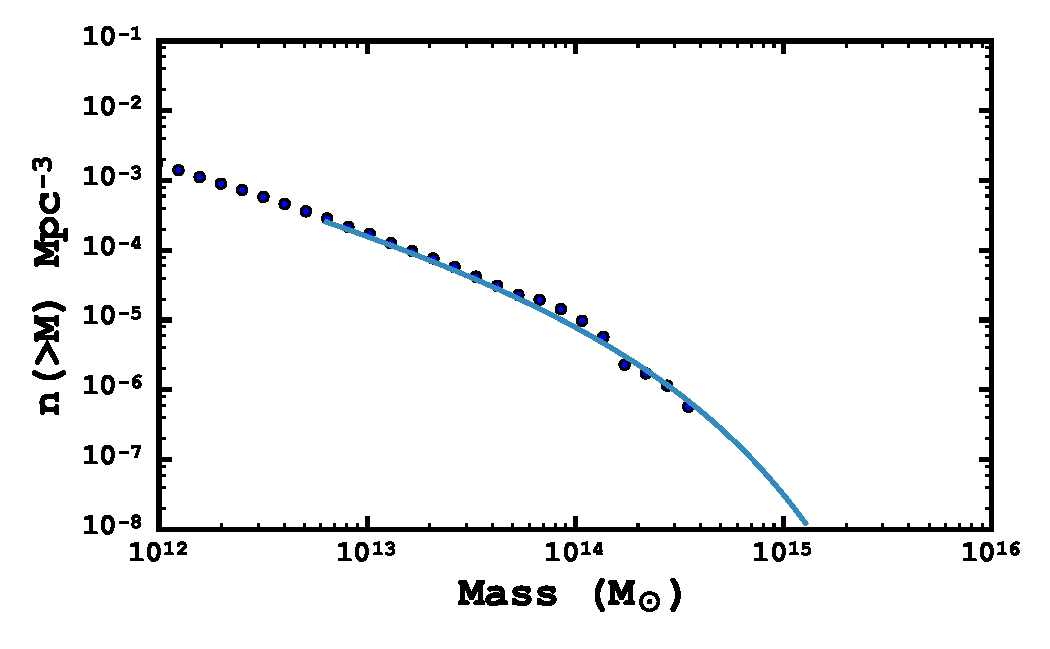
\includegraphics[width=\columnwidth]{figures/hmf.pdf} 
	\caption{The cumulative MF (from \citealt{Tinker2008}) of halos above $M_{200c}$ at $z=0.1$} 
	\label{fig: hmf} 
\end{figure}

We investigate the accuracy of the halo mass distribution by comparing the cumulative number density of halos above a mass ($M_{200c}$) threshold to the halo mass function (HMF) of \cite{Tinker2008}. Shown in Figure~\ref{fig: hmf} the HMF is calculated at central redshifts of 0, 0.2, and 0.4 using {\tt HMFcalc} \citep{Murray2013} and compared to galaxies in a redshift window of $\Delta z\pm0.01$. We find a very good agreement between the expected HMF and the observed. 

\subsection{ {\rm[\ion{O}{ii}]} Luminosity}\label{sec: oii luminosity}
\begin{figure*} 
	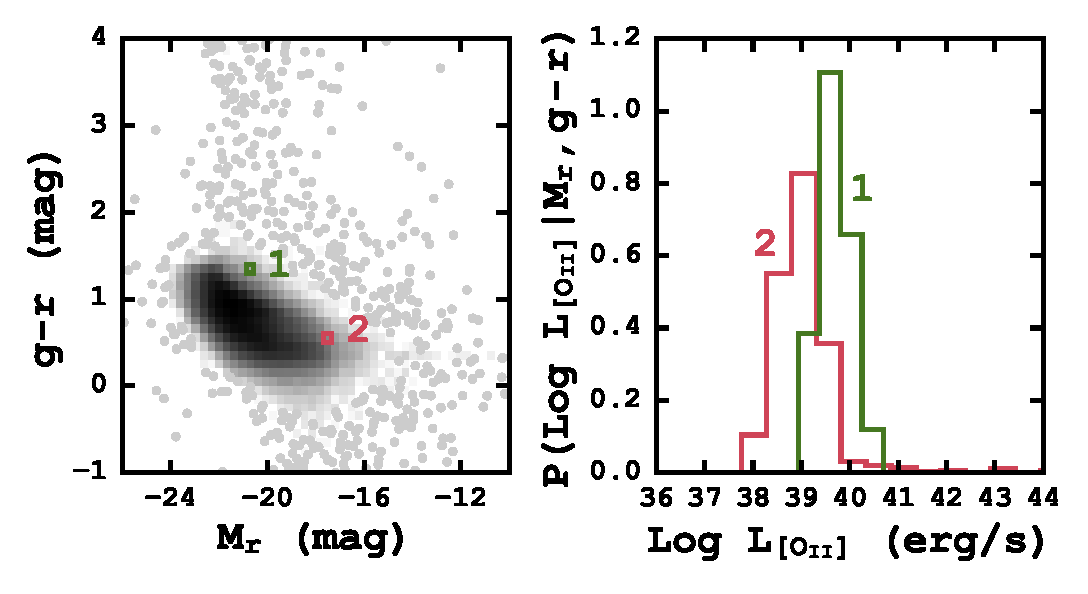
\includegraphics[width=\textwidth]{figures/oii_sdss.pdf} 
	\caption{\textit{Left}: CMD of 503113 $z<0.2$ galaxies take from the SDSS DR12 where the shading scales with the density of points. The two boxes show regions containing potential catalog galaxies. \textit{Right}: Probability histograms of the Log [\ion{O}{ii}] luminosity for the SDSS galaxies located in the two highlighted regions on the right. New [\ion{O}{ii}] luminosity (and subsequently fluxes) are assigned to catalog galaxies from slice sampling the probability histogram.} \label{fig: oii sdss} 
\end{figure*}

The Buzzard ``truth'' catalog does not provide [\ion{O}{ii}] luminosities so we must assign them empirically. We use 503113 galaxies from the SDSS Data Release 12 \citep{Alam2015} from $z = 0.05 - 0.2$, which are selected with no redshift warning, and place each galaxy on a color-magnitude diagram (CMD) of $M_r$ and $g-r$, see Figure~\ref{fig: oii sdss}.

To assign an [\ion{O}{ii}] luminosity to each galaxy in our catalog we place the catalog galaxies on the same CMD and select all SDSS galaxies in a small 2D ($M_r$, $g-r$) bin around the galaxy. We extract all of the SDSS galaxies inside that bin and create a histogram of their [\ion{O}{ii}] luminosities. Using a slice sampling technique \citep{Neal1997} we assign the catalog galaxy an [\ion{O}{ii}] luminosity based on the distribution of SDSS galaxies extracted. For catalog galaxies which are placed on the CMD near no, or very few ($1\leq n<10$) galaxies we assign it zero [\ion{O}{ii}] luminosity or the mean luminosity, respectively.

The right panel of Figure~\ref{fig: oii sdss} shows the CMD of all SDSS galaxies. Two potential catalog galaxies are also placed on the CMD ($M_r, g-r = -17.7,~0.49$ and $M_r, g-r = -21.4,~1.24$) and indicated by two colored boxes. The histograms show in the Figure's left panel shows the probability density histograms of the Log [\ion{O}{ii}] luminosity for the SDSS galaxies in the 2D bin. We sample the distribution and assign each catalog galaxy an [\ion{O}{ii}] luminosity which is then converted into a flux.

\subsection{Mock Observations}\label{sec: observations}
\editorial{Not sure this does a good enough job talking about the two different observations.}
Tentatively slated to start in the spring of 2016, HETDEX will perform blind spectroscopy (R $\sim$ 750 in $3500 - 5500~\AAA$) over two fields along the celestial equator. The 300 \degsq, spring field and 120 \degsq, fall field will have no preselected targets. Using VIRUS on the 10-m Hobby-Eberly Telescope (HET; \citealt{Ramsey1998}) the completed survey is expected to have an overall fill-factor of 1/4.5, meaning that the entire area could be covered with 4.5 dithers of the entire survey. 

The spectral coverage allows for the detection of [\ion{O}{ii}] ($\lambda\lambda 3727-3729~\AAA$ doublet) emitters to $z\sim 0.5$ and Ca H ($\lambda 3968.5~\AAA$) and K ($\lambda 3933.7~\AAA$) absorption features to $z\sim 0.4$. HETDEX is expected to detect sources with continuum brighter than 22 mag in \sdssg, and emission line strengths above $3.5\times10^{-17}$ \ergscm. So we ``observe'' $z<0.4$ galaxies which meet either the emission line or the magnitude limit. Galaxies $0.4<z<0.5$ are only observed if their emission line strength is sufficient. \editorial{These limits have been changed. FIX!}

\begin{figure} 
	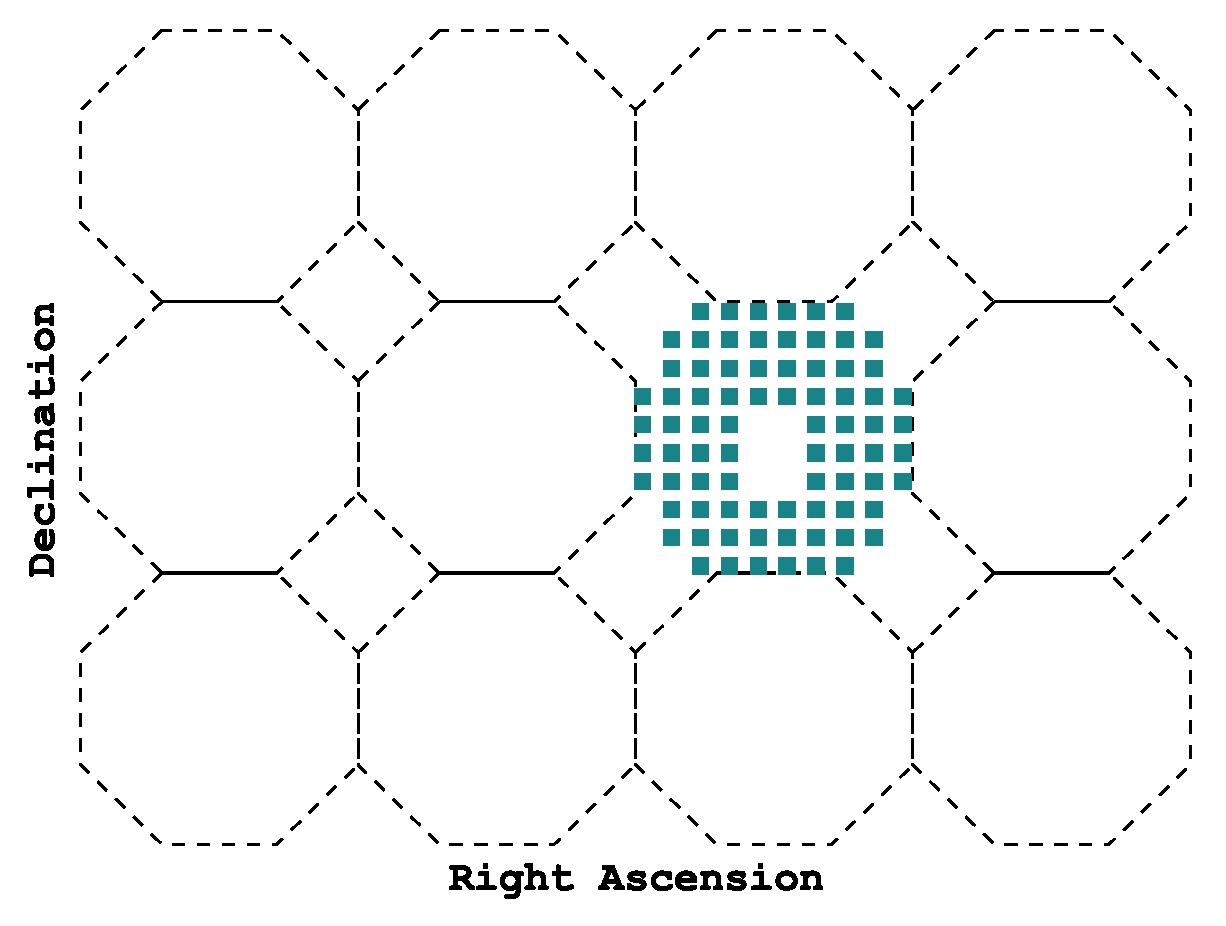
\includegraphics[width=\columnwidth]{figures/f01.pdf} 
	\caption{Representative observation tiling scheme for the HETDEX $16' \times 16'$ pointings. Each colored square is a single VIRUS IFU and the dashed octagons approximate the size of a single observation. See the text for more details.} \label{fig: ifu layout} 
\end{figure}

In this work we consider two separate observation cases. The first are targeted observations where we select each galaxy cluster and ``observe'' each galaxy within $8'$ of the center. The second is a survey case where observations which are blind to the positions of the clusters are conducted. In both cases, our ``observations'' consist of placing masks down onto the Buzzard ``truth'' catalogs and selecting all, $z< 0.5$ also meeting sensitivity limits, galaxies which lie underneath. Each mask is created to accurately reproduce the HETDEX IFU pattern, see Figure~\ref{fig: ifu layout}. The pattern consists of 78 IFUs, which are comprised of 448 optical fibers subtending a $50'' \times 50''$ region on the sky \citep{Kelz2014}. The inter-IFU spacing is also $50''$ spanning a total area of $16'\times 16'$ on the sky. 

The individual IFUs have a fill-factor of 1/3, which will be completely filled with three dithers of the telescope at each pointing. This means that when selecting galaxies from the Buzzard catalog we assume an observation for all galaxies laying within a colored, IFU square in Figure~\ref{fig: ifu layout}. \editorial{This should be updated with the fiber collisions.} Galaxies which lie between the IFUs are missed, as well as the galaxies which lie between the pointings, as there is no overlap between one pointing and the next. To cover the 375.67 \degsq\ field of the Buzzard catalog we require 5370 pointings where 0.015 \degsq\ of each pointing is covered by an IFU. The total area of the sky covered by an IFU is 80.80 \degsq\ which gives a filling factor of 1/4.65 slight decreased from the expected filling factor of 1/4.5. 

\section{Recovery of Parameters}\label{sec: recovery}
 In the following sections, we outline the methods we use to derive the dynamical properties of the galaxy clusters in our sample. This is not meant to be an exhaustive study of the different methods used to recover these parameters. The following is, in many cases, a subset of the available methods to derive any single parameter. The specific choice of method may improve or diminish the accuracy of the recovered parameter, but the methods chosen were to facilitate comparison with observational studies. 

\subsection{Cluster Redshift}
The accurate determination of the cluster redshift ($z_c$) is crucial to the reliability of all following measurements. An incorrect cluster redshift introduces errors into the measured line-of-sight velocity (LOSV) and corresponding dispersion, which, in turn, contributes to errors associated with dynamical mass and radius. 

In simple terms, the cluster redshift is the mean of the redshifts of all galaxies associated with the cluster. However, because the standard mean can be quite sensitive to outliers or otherwise contaminated data, we require a more resistant statistic, and turn to the biweight location estimator \citep{Beers1990} which provides improved performance. 

\subsection{Line-of-Sight Velocity Dispersion}\label{sec: LOSVD}
We first calculate the line-of-sight velocity (LOSV) to each galaxy, where
\begin{equation}
	LOSV = c\frac{z - z_c}{1+z_c}
\end{equation}
and $c$ is the speed of light in \kms, $z$ is the redshift of the individual galaxy, and $z_c$ is the overall cluster redshift described in the previous section.

The line-of-sight velocity dispersion (LOSVD) is calculated using a method of maximum likelihood following \cite{Walker2006}. We maximize the probability function 
\begin{equation}
  \label{eq: jointGaussian}
p(\{v_1, ..., v_N\})=\displaystyle\prod_{i=1}^{N}\frac{1}{\sqrt{2\pi(\sigma_i^2+\sigma_p^2)}}\exp\biggl[-\frac{1}{2}\frac{(v_i-\langle u \rangle)^2}{(\sigma_i^2+\sigma_p^2)}\biggr]
\end{equation}
where $\sigma_p$, $\langle\mu\rangle$, and $\sigma_i$ is the LOSVD, the average radial velocity and the error on the individual LOSVs respectively. Using a Monte Carlo Markov Chain sampler ({\sc emcee}\footnote{\url{http://dan.iel.fm/emcee/current/}}, \citealt{Foreman-Mackey2013}), we draw twenty thousand samples from the posterior probability distribution. Simple priors, $\langle\mu\rangle$ lies between the maximum and minimum LOSV and $0< \sigma_p$, are used. When the full distribution of LOSVDs are not used, the final LOSVD is quoted as the median value of the probability distribution with 68\% error bars defined as the 16th and 84th percentiles of the same distribution.

In principle, a single statistic such as the biweight scale estimator or the gapper estimator (both from \citealt{Beers1990}) with many bootstrap resamplings could be used to construct a distribution of $\sigma_p$. We prefer the maximum likelihood method for its straight forward treatment of the errors in the LOSV measurements. \editorial{Maybe run a quick check to see how they compare.}

\subsection{Dynamical Mass}\label{sec: mass}
Recently, the relationship between the LOSVD and dynamical mass has been the focus of several studies \citeeg{Evrard2008, Saro2013, Sifon2013, VanderBurg2014}, and a best fitting relationship for the mass enclosed by $r_{200c}$ of the form
\begin{equation}\label{eq: mass scaling}
	M_{200c} = \frac{10^{15}}{h(z)} \bigg{(}\frac{\sigma_{1D}}{A_{1D}} \bigg{)}^{1/\alpha} \Msol
\end{equation}
with $A_{1D} = 1177 \pm 4.2$ \kms\ (\citealt{Munari2013}; referred to as $\sigma_{15}$ in \citealt{Evrard2008} and other works), $\alpha = 1/3$, $h(z) = H(z)/100$, and $\sigma_{1D}$ is the LOSVD of the velocity tracers (dark matter particles, subhalos or galaxies). 

A growing body of work suggests that there is a significant difference in the observed LOSVD depending on the velocity tracers used. Specifically, while there is little difference between using galaxies and their host DM subhalos, there is a significant over estimation of the LOSVD when using galaxies/subhalos compared to DM particles \citep{Munari2013}. We follow other works \citeeg{Kirk2015, Sifon2015a} using the scaling relation, given in Equation~\ref{eq: mass scaling} from \cite{Munari2013} to facilitate comparisons with other observational studies. 
% \editorial{This all needs to be stripped out and reworked.}
% The choice $A_{1D}$ and $\alpha$ varies between studies \citeeg{Munari2013, VanderBurg2014} and should be calibrated on a individual basis. To do this, we randomly select 47494, $z<0.5$ clusters composed of 36000 $10^{13}$, 6000 $10^{14}$ and two $10^{15}~\Msol$ halos. We perform a linear fit to the $\sigma_{1D}-M_{200}$ values allowing both $A_{1D}$ and $\alpha$ to vary. We find best fitting parameters of $A_{1D} = 1117.9~\kms$ and $\alpha = 0.3297$, both of which are very near the values from \cite{Evrard2008} of $A_{1D} = 1082.9 \pm 4.0~\kms$ and $\alpha = 0.3361$. Therefore, we chose to adopt the parameters from \cite{Evrard2008} to better facilitate with other simulations \citeeg{Old2014}, and observational studies \citeeg{Brodwin2010}.

\subsection{Dynamical Mass Corrections}
In this section we use two methods to predict the mass of a cluster based on other observables. Often the cluster mass is estimated based on a single observable, X-ray temperature, velocity dispersion, richness and others. Here we combine many observables to attempt to correct the mass inferred solely from the velocity dispersion. The first method is traditional probability based where we marginalize over a series of observables to find the most probable mass. The second is based on a machine learning (ML) algorithm which attempts to ``learn'' the relationship between the observables and the desired output, the mass. Both of these methods are examples of supervised learning algorithms where the relationship between the observable (known) parameters and the target parameter (the mass) are both known.

As with any predictive analysis it is important to test the model on data that the model has not seen before. In this section we take all of the observed clusters, our full sample, split them, and generate a training and testing set. The data is randomly split 70\% training and 30\% testing. We follow the ML convention and refer to the individual clusters in each set as a ``sample'', and the parameters associated with the cluster ($z$, LOSVD, mass, etc.) as ``features''.  

\subsubsection{Probability Based}\label{sec:probability method}
We begin with the training sample. After selecting the desired features $\vec{x} = \{\sigma, z, ...\}$ we make the joint probability between the true cluster mass (M) and $\vec{x}$. Because $\vec{x}$ can be multidimensional, we rely on the corner plot to visualize the relationship between all of the training features. Figure~\ref{fig: probability corner} shows all of the one (marginalized probability) and two (joint probability) dimensional projections of the posterior probability distributions of the features of the training data.

\begin{figure} 
	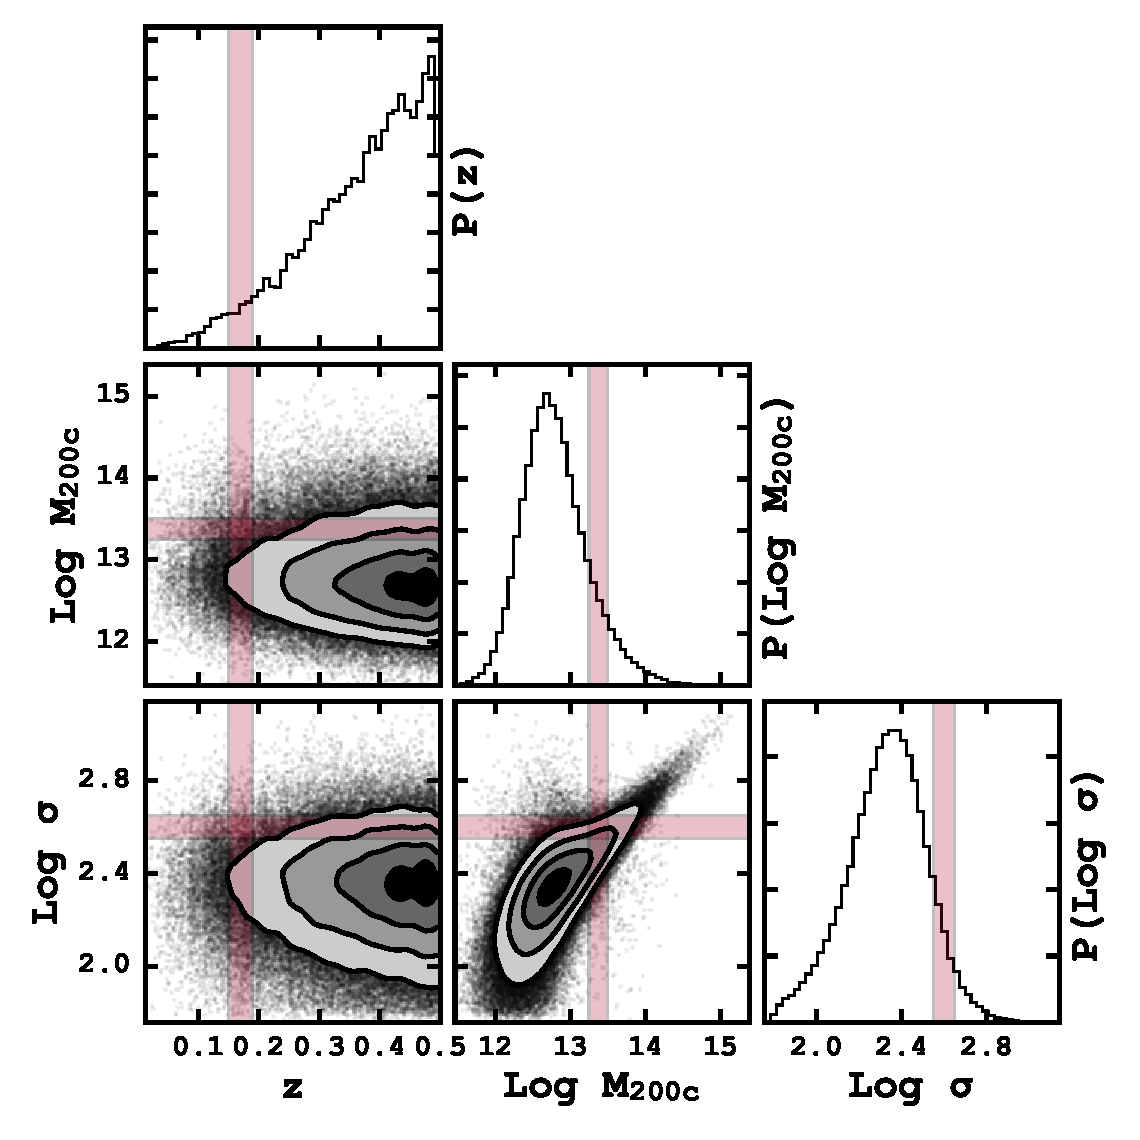
\includegraphics[width=\columnwidth]{figures/cornertest.pdf} 
	\caption{Corner plot of the \emph{training} data with features $\sigma$ and $z$. The corner plots shows all of the one and two dimensional posterior probability distributions used to determine the correct cluster mass. The colored rectangles show the slices needed to create a conditional probability distribution of the mass, $P(M|\vec{x})$. See text for a complete description. } \label{fig: probability corner} 
\end{figure}

The conditional probability of the mass $P(M|\vec{x}= \{ x_1,x_2,...\})$ is determined by taking a slice through the joint probability distributions in bins centered on the desired value. The slices show by the colored bars in Figure~\ref{fig: probability corner} are centered on $\sigma = 500$ \kms and $z=0.17$. The distribution of mass contained in the three dimensional bin given by the intersection of these slices is $P(M|\vec{x} = \{ \sigma=500 \kms,z=0.17\})$.

For the clusters making up the \emph{test} sample the mass is unknown (it is what we are trying to predict) but the other features are known. To determine the mass probability distribution of a test cluster, $P(M)$ we combine the conditional probability distribution, $P(M|\vec{x})$, created previously with the probability distribution of $\sigma$ through Equation~\ref{eq: Pm}.
\begin{equation}\label{eq: Pm}
	P(M) = \int P(M|\vec{x}) P(\sigma) d\sigma
\end{equation}
The expected mass is determined by integrating the mass probability, $P(M)$ over all mass. This becomes our ``predicted'' mass, $\langle M\rangle$.
\begin{equation}\label{eq: expected mass}
	\langle M\rangle = \int M^\prime P(M^\prime)dM^\prime
\end{equation}
The confidence interval associated with this prediction can be estimated two ways. First, by calculating the variance about the expected mass through
\begin{equation}\label{eq: variance}
	V = \int (M^\prime - \langle M\rangle)^2 P(M^\prime)dM^\prime
\end{equation}
or by drawing many samples from $P(M)$ and calculating the values at the 16th and 84th percentile. In practice we find that both methods produce similar results for a large number of trials. Therefore, we quote predicted masses as the most probable mass given by Equation~\ref{eq: expected mass} and associated 68\% error estimated through Equation~\ref{eq: variance}.

\subsubsection{Machine Learning Based}\label{sec:machine learning method}
The estimation in this section relies on a ML technique known as an ensemble method, where many estimators are created by a single learning method with the goal of improved generalization and robustness compared to a single estimation. Ensemble methods come in two general flavors. Averaging methods average (hence the name) the estimators to produce a single prediction. Boosting estimators build estimates sequentially by attempting to address poor performing estimators in each previous step, hence ``boosting'' the predictive power.

Here we use an averaging ensemble learning method known as a forest of randomized decision trees often shorten to just random forest (RF). Decision trees can be visualized a flow chart where forks are the branches of the tree. The path along the tree is decided by the values of the feature at each branch. RF estimators use a random subset of the training set at each fork to decide which path should be followed. The final prediction is then the average of all the trees. We use RF regression methods as implemented in {\tt Scikit-Learn} \citep{Pedregosa2012}.

The 68\% prediction interval is determined by calculating the 16th and 84th percentile of all the predictions made by the ensemble of estimators.

\section{RESULTS}\label{sec: results}
Here we explore the cluster member recovery rate and mass estimates for the two observing strategies. We discuss the accuracy of dynamical mass derived from both the scaling relation (see Equation~\ref{eq: mass scaling}) and through the probability and ML methods.

\subsection{Recovery of Cluster Members}
As discussed in Section~\ref{sec: observations} the observational constraints place limits on the total number fo clusters member galaxies expected to be recovered. Knowing these limits will provide important information for potential future follow up or targeted observations. 

\begin{figure*} 
	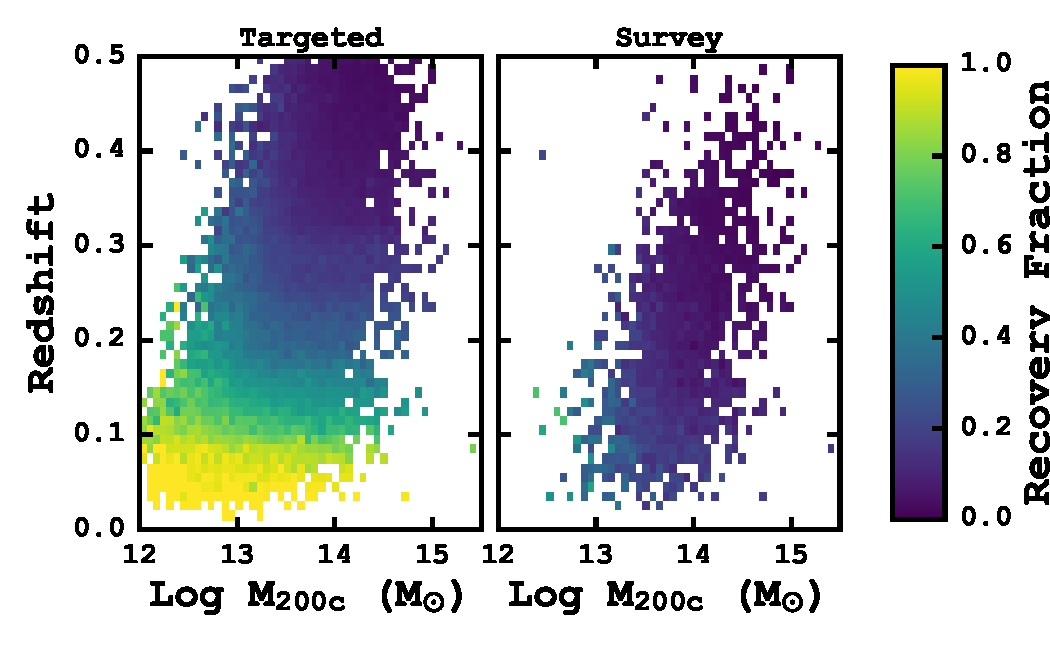
\includegraphics[width=\textwidth]{figures/recovery.pdf} 
	\caption{Recovery fractions ($N_{obs}/N_{True}$) of cluster member galaxies as a function of redshift and mass for the targeted (upper row) and survey (lower row) observing strategies. The significant decline in galaxies observed with the survey strategy is due to gaps in the VIRUS IFU.} \label{fig: recovery} 
\end{figure*}

Figure~\ref{fig: recovery} shows the recovery fraction of member galaxies, the number of observed versus the number of actual galaxies, as a function of both redshift and cluster mass for the targeted and survey observing strategies. As expected, the targeted observing strategy where the individual clusters are targeted through several dithers to ensure near complete coverage, performs significant better than the survey observing strategy for nearly all redshifts and cluster masses. This performance gain is due solely to the gaps between the fiber bundles of the IFU. 

\editorial{why does the recovery fraction decrease with redshift? Are the clusters smaller? Do they not have as many galaxies per cluster at higher redshifts? Is it a magnitude effect? I also want to add an error bar estimation for several of the percentages to give a feel for how the different recovery levels effect the accuracy of the measurements.}

\subsection{Mass estimates}
In this section we discuss the how accurately we are able to reproduce the true cluster mass from a set of observations. We report on two methods the probability based approach (Section \ref{sec:probability method}) and the machine learning based method (Section \ref{sec:machine learning method}). For each method we consider both targeted and HETDEX-like observing strategies.

All of the figures presented here show the predicted versus true cluster masses for one of the two observing strategies. In each panel the solid black line shows the 1:1 relationship, the colored, solid line is the median recovered mass, and the shaded region is the 68\% scatter of the cluster masses. The lower panels show the fractional mass error: 
\begin{equation}\label{eq: fractional error}
	\epsilon = (M_{pred} - M)/M
\end{equation}
where $M_{pred}$ is the predicted cluster mass and $M$ is the true cluster mass.

\subsubsection{Probability Based}
Figures \ref{fig:Probability comparison_survey} and \ref{fig:Probability comparison} show the power law predictions compared to the predictions based on probability propagation. 

\begin{figure*} 
	\includegraphics[width=\textwidth]{figures/MLcomparison_survey.pdf} 
	\caption{Mass predictions for the power law scaling relation (Equation~\ref{eq: mass scaling}) and the ML technique with different input features. The bottom row of panels shows the fractional error (Equation~\ref{eq: fractional error}) as a function of mass. The solid black line shows the 1:1 relation. The colored lines and shaded region show the median value and 68\% bounds respectively.} \label{fig:Probability comparison_survey} 
\end{figure*}

\begin{figure*} 
	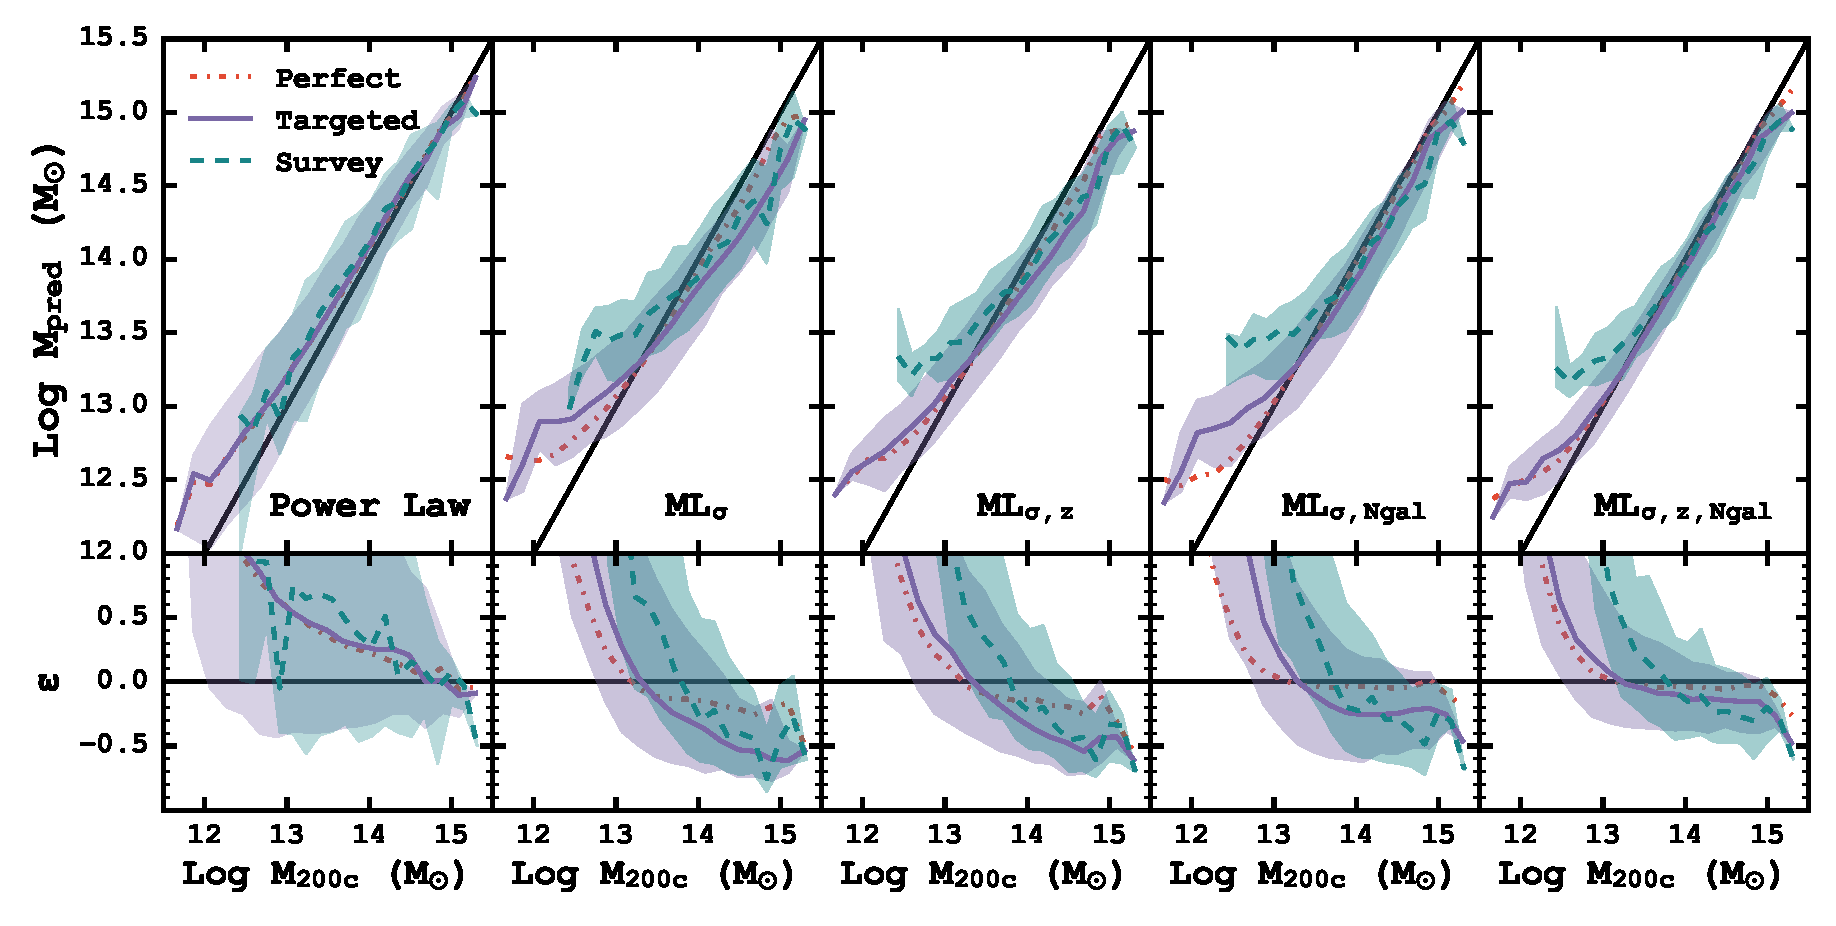
\includegraphics[width=\textwidth]{figures/MLcomparison.pdf} 
	\caption{Mass predictions for the power law scaling relation (Equation~\ref{eq: mass scaling}) and the ML technique with different input features. The bottom row of panels shows the fractional error (Equation~\ref{eq: fractional error}) as a function of mass. The solid black line shows the 1:1 relation. The colored lines and shaded region show the median value and 68\% bounds respectively.} \label{fig:Probability comparison} 
\end{figure*}



\subsubsection{Machine Learning Based}
Figures \ref{fig: ML comparison_survey} and \ref{fig: ML comparison} show the power law predictions compared to the RF predictions using LOSVD ($\sigma$) combined with both $z$ and the number of galaxies observed, $N_{gal}$.  

\begin{figure*} 
	\includegraphics[width=\textwidth]{figures/MLcomparison_survey.pdf} 
	\caption{Mass predictions for the power law scaling relation (Equation~\ref{eq: mass scaling}) and the ML technique with different input features. The bottom row of panels shows the fractional error (Equation~\ref{eq: fractional error}) as a function of mass. The solid black line shows the 1:1 relation. The colored lines and shaded region show the median value and 68\% bounds respectively.} \label{fig: ML comparison_survey} 
\end{figure*}

\begin{figure*} 
	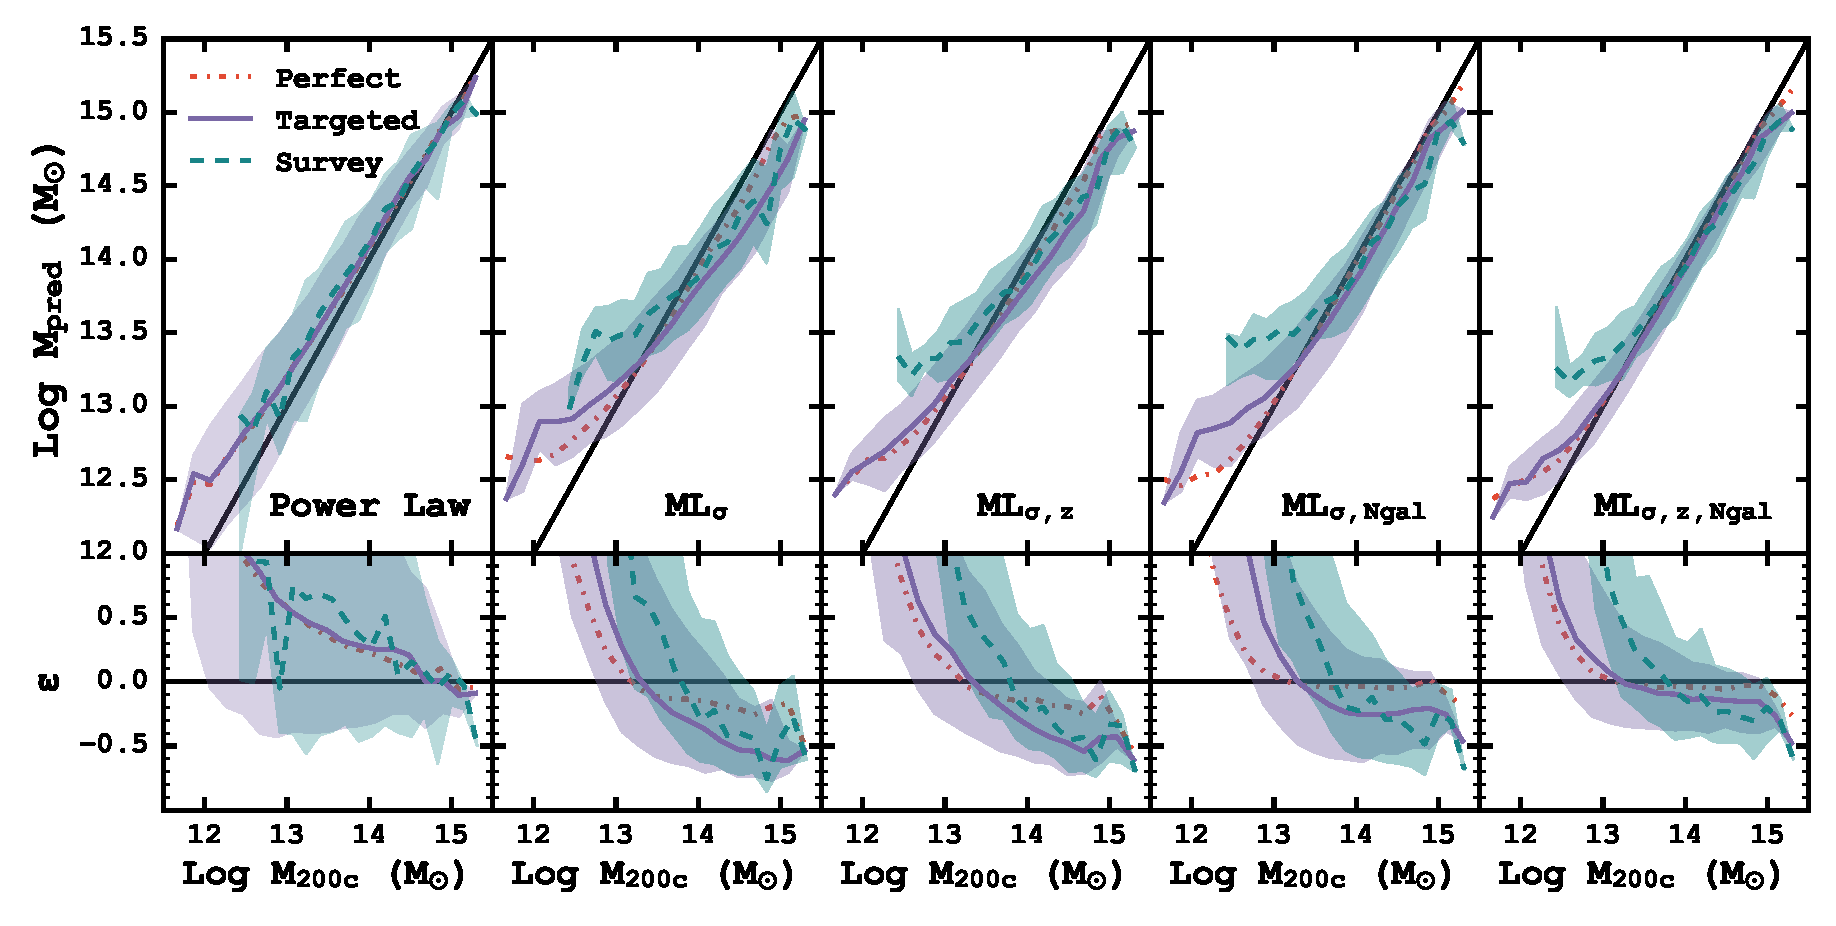
\includegraphics[width=\textwidth]{figures/MLcomparison.pdf} 
	\caption{Mass predictions for the power law scaling relation (Equation~\ref{eq: mass scaling}) and the ML technique with different input features. The bottom row of panels shows the fractional error (Equation~\ref{eq: fractional error}) as a function of mass. The solid black line shows the 1:1 relation. The colored lines and shaded region show the median value and 68\% bounds respectively.} \label{fig: ML comparison} 
\end{figure*}

% \editorial{It doesn't look like you can use the targeted training sample to train the survey data. If you do, it either does worse or about the same if you didn't use any training at all. After looking at it, you do have to use the survey training data to get good results about 0.13 dex MAE
% }

\section{HETDEX as a Galaxy Cluster Survey}

\subsection{Expected Results}
Lorem ipsum dolor sit amet, consectetur adipisicing elit, sed do eiusmod tempor incididunt ut labore et dolore magna aliqua. Ut enim ad minim veniam, quis nostrud exercitation ullamco laboris nisi ut aliquip ex ea commodo consequat. Duis aute irure dolor in reprehenderit in voluptate velit esse cillum dolore eu fugiat nulla pariatur. Excepteur sint occaecat cupidatat non proident, sunt in culpa qui officia deserunt mollit anim id est laborum.

\subsection{Potential Improvements}
Lorem ipsum dolor sit amet, consectetur adipisicing elit, sed do eiusmod tempor incididunt ut labore et dolore magna aliqua. Ut enim ad minim veniam, quis nostrud exercitation ullamco laboris nisi ut aliquip ex ea commodo consequat. Duis aute irure dolor in reprehenderit in voluptate velit esse cillum dolore eu fugiat nulla pariatur. Excepteur sint occaecat cupidatat non proident, sunt in culpa qui officia deserunt mollit anim id est laborum.

\subsection{Extendability to Other Surveys}
Lorem ipsum dolor sit amet, consectetur adipisicing elit, sed do eiusmod tempor incididunt ut labore et dolore magna aliqua. Ut enim ad minim veniam, quis nostrud exercitation ullamco laboris nisi ut aliquip ex ea commodo consequat. Duis aute irure dolor in reprehenderit in voluptate velit esse cillum dolore eu fugiat nulla pariatur. Excepteur sint occaecat cupidatat non proident, sunt in culpa qui officia deserunt mollit anim id est laborum.

\section{SUMMARY}
Lorem ipsum dolor sit amet, consectetur adipisicing elit, sed do eiusmod tempor incididunt ut labore et dolore magna aliqua. Ut enim ad minim veniam, quis nostrud exercitation ullamco laboris nisi ut aliquip ex ea commodo consequat. Duis aute irure dolor in reprehenderit in voluptate velit esse cillum dolore eu fugiat nulla pariatur. Excepteur sint occaecat cupidatat non proident, sunt in culpa qui officia deserunt mollit anim id est laborum.

\section*{Acknowledgements}
The authors also wish to thank the anonymous referee whose comments and suggestions significantly improved both the quality and clarity of this work. We also thank Steven W. Crawford for many helpful discussions. This research made use of This research made use of  the {\tt IPython} package \citep{Perez2007} and {\tt matplotlib}, a Python library for publication quality graphics \citep{Hunter2007}. Funding for the SDSS and SDSS-II has been provided by the Alfred P. Sloan Foundation, the Participating Institutions, the National Science Foundation, the U.S. Department of Energy, the National Aeronautics and Space Administration, the Japanese Monbukagakusho, the Max Planck Society, and the Higher Education Funding Council for England. The SDSS Web Site is http://www.sdss.org/. The SDSS is managed by the Astrophysical Research Consortium for the Participating Institutions.

%%%%%%%%%%%%%%%%%%%% REFERENCES %%%%%%%%%%%%%%%%%%
% The best way to enter references is to use BibTeX:
\bibliographystyle{mnras}
\bibliography{master} % if your bibtex file is called example.bib

%%%%%%%%%%%%%%%%% APPENDICES %%%%%%%%%%%%%%%%%%%%%
% \appendix
%
% \section{Some extra material}
%
% If you want to present additional material which would interrupt the flow of the main paper,
% it can be placed in an Appendix which appears after the list of references.

% Don't change these lines
\bsp	% typesetting comment
\label{lastpage}
\end{document}

% \begin{equation}
%     x=\frac{-b\pm\sqrt{b^2-4ac}}{2a}.
% 	\label{eq:quadratic}
% \end{equation}
%
% % Example figure
% \begin{figure}
% 	% To include a figure from a file named example.*
% 	% Allowable file formats are eps or ps if compiling using latex
% 	% or pdf, png, jpg if compiling using pdflatex
% 	\includegraphics[width=\columnwidth]{example}
%     \caption{This is an example figure. Captions appear below each figure.
% 	Give enough detail for the reader to understand what they're looking at,
% 	but leave detailed discussion to the main body of the text.}
%     \label{fig:example_figure}
% \end{figure}
%
% % Example table
% \begin{table}
% 	\centering
% 	\caption{This is an example table. Captions appear above each table.
% 	Remember to define the quantities, symbols and units used.}
% 	\label{tab:example_table}
% 	\begin{tabular}{lccr} % four columns, alignment for each
% 		\hline
% 		A & B & C & D\\
% 		\hline
% 		1 & 2 & 3 & 4\\
% 		2 & 4 & 6 & 8\\
% 		3 & 5 & 7 & 9\\
% 		\hline
% 	\end{tabular}
% \end{table}

% \section{Evidence of Substructure}
% Like the recovery of dynamical parameters discussed in the previous section, the choice of method to investigate the dynamical state of galaxy clusters is heavily debated. Perhaps the most widely used metric is the Dressler-Shectman (DS) test \citep{Dressler1988}, and is not without criticism \citeeg{White2010}. New methods such as the Caustic Method (\citealt{Yu2015}, and the references therein) offer promise to shed further light on this difficult problem.
%
% \subsection{From VD profiles}
% We utilize the modality \citep{Oliva-Altamirano2014} which describes the Gaussianity of a LOSV distribution in a galaxy cluster. For clusters with Gaussian distributed LOSVs, the modality is close to 1/3. It is defined as $(1+\mathrm{skewness}^2)/(3+\mathrm{kurtosis}^2)$. \editorial{Do I need to describe what the skewness and kurtosis is?}
%
% \subsection{Dominance}
% \editorial{This is taken pretty directly from the GAMA paper. Will need to be edited to fit.}
% The dominance is defined as the luminosity gap between the brightest and the second brightest galaxy in a cluster ($\Delta m_{1, 2}$). The amplitude of the luminosity gap between the BGG/BCG and the second brightest galaxy in the halo, is expected to be a function of both the formation epoch and the recent infall history of the halo. A small magnitude gap ($\Delta m_{1, 2} < 1$) indicates a recent halo merger, and larger gaps ($\Delta m_{1, 2} > 1$), common in fossil groups, is perhaps indicative of a cluster or groups that has not undergone a recent merger.
%
% \subsection{Dressler-Schectman Test}
% We leverage the large spectroscopic dataset to study the structural properties of the clusters. \cite{Pinkney1996} determine, from a comparison of five different methods that the DS test is the most sensitive to the presence of substructure.
%
% The DS test, which combines the spatial positions and velocities of the galaxies, provides a method to locate substructure by identifying groups of galaxies which differ significantly from the cluster velocity distribution. Galaxy subsets are selected from a cluster of $n_{members}$ and each constituent galaxy deviation is calculated according to
% \begin{equation}
% 	\delta_i^2 = \frac{N_{local}+1}{\sigma^2}\bigg{[}(\bar{v}_{local,i} - \bar{v})^2 + (\sigma_{local,i} - \sigma)^2\bigg{]}^2
% \end{equation}
% where $\bar{v}_{local}$ and $\sigma_{local}$ are the mean velocity and velocity dispersion for a subset of $N_{local}$ galaxies and $\bar{v}$ and $\sigma$ are the entire cluster's mean velocity and velocity dispersion. The choice of $N_{local}$ is left to the user. Originally, \cite{Dressler1988} choose $N_{local}=10$, however \cite{Bird1994} points out that using a fixed value for $N_{local}$ reduces the sensitivity to substructure. We follow \cite{Bird1994} in choosing $N_{local} = \sqrt n_{members}$. \editorial{doesn't talk about the nearest neighbors which is what we are using.}
%
% The DS statistic is the $\Delta$-value given by,
% \begin{equation}
% 	\Delta = \sum^{n_{members}}_i \delta_i
% \end{equation}
% where a system is considered to contain substructure if $\Delta/n_{members} > 1$ \citep{Dressler1988}. A second method, described in \cite{Hou2012}, uses probabilities (P-values) rather than a threshold for the identification of substructure. P-values are computed by comparing the observed $\Delta$-value and the $Delta$-value after the velocities (but not positions) have been shuffled through a series of Monte Carlo runs. The probability of the existence of substructure becomes
% \begin{equation}
% 	P = \sum (\Delta_{shuffled} > \Delta_{Observed}) / n_{shuffle}
% \end{equation}
% where $n_{shuffle}$ is the number of shufflings used. \editorial{This sounds a whole lot like the description given in Hou2012. Make sure that we aren't copying anything word for word. That'd be bad.}
%
% In practice, we use locate the nearest neighbors using an unsupervised k-nearest neighbor algorithm as implemented in Scikit-Learn \citep{Pedregosa2012}.
